\begin{frame}{Các bước trong đường ống dữ liệu Pháp Điển}

\begin{figure}[H]
\centering
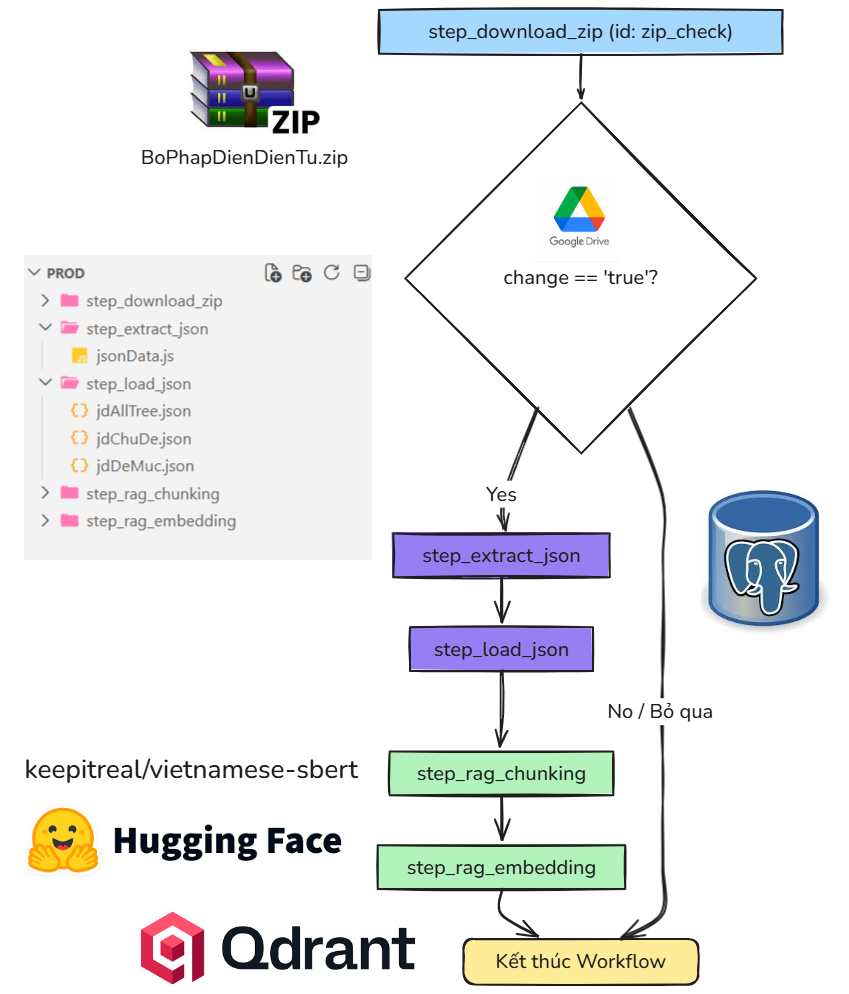
\includegraphics[width=\linewidth,height=0.74\textheight,keepaspectratio]{pictures/step3.excalidraw.png}
\caption{Sơ đồ các bước thực hiện của đường ống dữ liệu Pháp Điển}
\end{figure}

\note{

Tiếp theo là Sơ đồ các bước thực hiện của đường ống dữ liệu Pháp Điển

\hrule

Bắt đầu từ việc tải file ZIP
\hrule

sau đó kiểm tra sự thay đổi trên google drive

\hrule

giải nén và trích xuất thông tin thành các file JSON

\hrule

VBPL thực hiện Chucking bằng LLM

còn pháp điển thực hiện Chucking theo chương

vì dữ liệu được chia các chương rõ ràng

\hrule

cuối cùng sử dụng mô hình nhúng embeddings

trên HuggingFace là vietnamese-sbert

thực hiện vector hóa để lưu vào cơ sở dữ liệu vector

}
\end{frame}

% tiếp theo là sơ đồ các bước thực hiện của đường ống dữ liệu pháp điển

% bắt đầu từ việc tải file zip, sau đó kiểm tra sự thay đổi trên google drive

% giải nén và trích xuất thông tin thành các file dây sừn

% văn bản pháp luật thực hiện chăng king bằng llm còn pháp điển thực hiện chăng king theo chương vì dữ liệu được chia các chương rõ ràng

% cuối cùng sử dụng mô hình nhúng embeddings trên húc ging phây là vietnamese-sbert thực hiện vector hóa để lưu vào cơ sở dữ liệu vector
